%\documentclass[9pt]{article}
\documentclass[article]{IEEEtran}
\usepackage{graphicx}
\usepackage{float}
\usepackage{amsmath}
\usepackage{amsfonts}
\usepackage[brazilian]{babel}
\usepackage[utf8]{inputenc}
\usepackage[backend=biber]{biblatex}
\usepackage{csquotes}
\usepackage{gensymb}
%\usepackage{docmute}
\usepackage{array}
\usepackage{multicol}
\usepackage{geometry}
\usepackage[T1]{fontenc}
\addbibresource{rel_parcial_erik_perillo_2sem2016.bib}

\newcommand{\fromeng}[1]{\footnote{do inglês: \textit{#1}}}
\newcommand{\tit}[1]{\textit{#1}}
\newcommand{\tbf}[1]{\textbf{#1}}
\newcommand{\ttt}[1]{\texttt{#1}}
\newcommand{\ie}{i.~e.~}
\newcommand{\eg}{e.~g.~}

\begin{document}

\newgeometry{margin=1.0in}

\begin{titlepage}
	\centering
	{\scshape\Large Relatório Parcial\par}
	\vspace{1.5cm}
	{\huge\bfseries Processos atencionais e aprendizado de máquina
		para sistemas robóticos\par}
	\vspace{1cm}
	{\itshape Aluno: Erik de Godoy Perillo\par}
	{\itshape Orientadora: Profa. Dra. Esther Luna Colombini\par}
	\vspace{0.5cm}
	\vfill
    Instituto de Computação\\
	Universidade Estadual de Campinas
	\vfill
	{\large \today\par}
\end{titlepage}

\newpage

%\begin{multicols}{2}
\section{Introdução}
A capacidade de percepção e construção de um modelo da realidade ao seu redor
é fundamental para que sistemas robóticos interajam com o ambiente e executem
tarefas diversas e complexas que podem ter as mais variadas utilidades para
os humanos.
Um componente fundamental para isso é a habilidade de dar foco apenas ao
relevante, evitando assim o processamento desnecessário de enormes quantias
de dados.

A atenção é um processo que faz parte do dia a dia de diversos seres vivos
em diversas maneiras e é razoável inspirar-se nela para a construção de
mecanismos semelhantes para a construção de sistemas de inteligência
artificial em máquinas.
Tal área tem sido foco de estudo há anos, resultando em diversas teorias
em psicologia sobre a atenção humana que inspiraram a implementação de
modelos computacionais bem sucedidos.

Neste trabalho, objetivamos construir um modelo atencional eficiente.
Com base no modelo, implementaremos um \tit{framework} atencional para
robôs móveis que permita o uso da seleção em tempo real dos estímulos
mais relevantes para as mais diversas tarefas que o robô possa executar.
No trabalho atual focamos na atenção visual, mas o objetivo
final do sistema é que ele funcione para outros sensores.
O \tit{framework} também contará com um módulo de reconhecimento de objetos
que poderá ser substituído.

\subsection{Objetivos da primeira parte do projeto}
Os objetivos principais para o primeiro semestre do trabalho eram:
\begin{itemize}
    \item Revisão bibliográfica sobre teorias sobre a atenção e diversos
        modelos.
    \item Escolha das técnicas mais adequadas para o processo atencional
        e o reconhecimento de objetos.
    \item Implementação de um modelo atencional.
\end{itemize}
Há uma quantidade surpreendente de avanços recentes na área de modelos
de saliência visual.
Entender os avanços mais relevantes é importante para a obtenção de um sistema
atencional eficiente, então foi requerido mais tempo que o previsto para
essa parte.
Assim, todas as etapas previstas tiveram avanço, com exceção da parte de
reconhecimento de objetos, a qual optamos por deixar para mais tarde pois
a mesma serve como um complemento para nosso trabalho e é de menor relevância
que o componente atencional.
As atividades desenvolvidas são mais detalhadas a seguir.

\section{Resumo das atividades}
\subsection{Revisão Bibliográfica}
Dois dos conceitos importantes para o entendimento da literatura do meio são:
\begin{itemize}
    \item \tit{features}: Características básicas que formam entidades
        visuais. Podem ser de várias classes, como cor
        (verde, azul), orientação (horizontal, vertical), luminância, tamanho.
    \item \tit{Bottom-up vs. Top-down}: Por componente \tit{bottom-up} de
        atenção entende-se saliências instintivas percebidas por mudanças
        e/ou contrastes muito grandes em uma cena. O componente \tit{top-down}
        é aquele que dá saliência variável às \tit{features} de acordo
        com a meta do agente do momento.
\end{itemize}
A maioria dos modelos computacionais baseia-se em teorias formadas na
psicologia.
Duas das mais famosas são a \tit{Feature Integration Theory}
(FIT)~\cite{TreismanGelade1980} e a
\tit{Guided Search}~\cite{Wolfe1989}.
Ambas provêm contribuiões importantes para o entendimento dos processos
de saliência visual.
Diversos modelos computacionais foram criados baseando-se em ideias delas.
Começou-se então por elas.

A FIT indica basicamente que se a busca de um objeto de interesse em uma
cena for por apenas uma \tit{feature}, a localização é feita em tempo
instantâneo.
Entretanto, se o objeto de interesse for composto por múltiplas \tit{features}
a serem buscadas (\eg uma linha horizontal verde),
a localização do objeto é feita em tempo linear.

Já \tit{Guided Search} diz que buscas por conjunções de \tit{features} são na
verdade mais rápidas pois a combinação das features gera um sinal de
saliência mais forte no campo visual humano.

O VOCUS~\cite{Frintrop2006} é um modelo atencional computacional
para a detecção de saliências visuais.
A maioria dos seus componentes é feita com base nas ideias da FIT\@.
Nesta primeira etapa, exploramos seu componente \tit{bottom-up}.
Ele lida com as \tit{features}: cor, intensidade, orientação.
Seus mapas de saliência são calculados com base nessas \tit{features}
e em diversas dimensões da imagem.

A revisão bibliográfica feita mostrou-se fundamental para os trabalhos
desenvolvidos no semestre.

\subsection{Modelo atencional}
A carga teórica adquirida foi útil para a concepção do nosso modelo,
chamado de \ttt{att}.
Muitos mecanismos foram inspirados no VOCUS, lidando com as mesmas
\tit{features} e em múltiplas dimensões da imagem.

\subsubsection{Extração de \tit{features}}
O modelo extrai os seguintes mapas de uma certa imagem:
luminância, luminância invertida, vermelho, verde, amarelo, azul,
orientações vertical, horizontal, 45\degree e 135\degree.
Os de luminância e cor podem ser extraídos pela conversão da imagem para o
espaço de cor LAB e as orientações são extraídas usando-se filtros de Gabor.

\subsubsection{Extração de saliência}
Para cada mapa, a saliência é calculada usando-se o mecanismo de
\tit{center-surround}~\cite{Frintrop2006}:
uma operação que basicamente extrai contrastes fortes
do mapa, dando intensidades de pixel altas para essas regiões.
O \tit{center-surround} pode ser aplicado por meio da convolução de um
\tit{kernel} apropriado na imagem.
Tal \tit{kernel} pode ter tamanho variado, mas a soma de seus valores deve
ser zero, o centro deve ter positivo e a vizinhança deve ter valores
negativos.
\begin{figure}[hbt]
\begin{center}
		\begin{tabular} {ccc}
            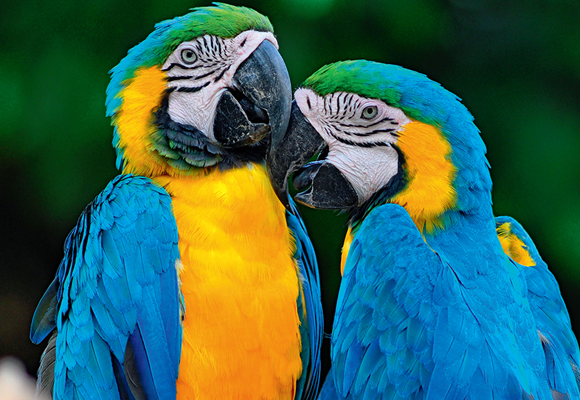
\includegraphics[width=0.3\linewidth]{img/arara.jpg}
            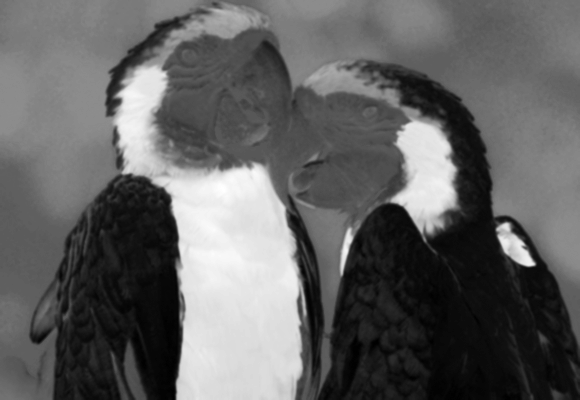
\includegraphics[width=0.3\linewidth]{img/arara_y.png}
            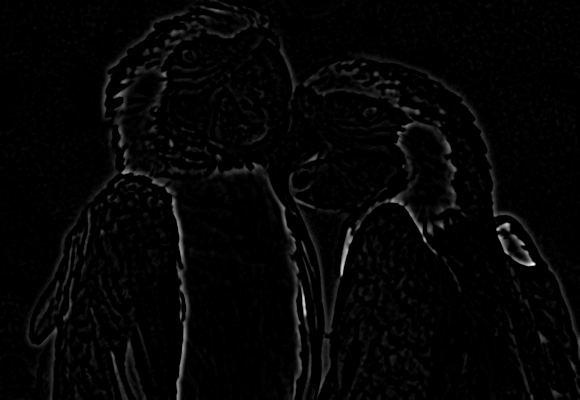
\includegraphics[width=0.3\linewidth]{img/arara_y_cs.png}
		\end{tabular}
\end{center}
\caption{À esquerda, a imagem original. No centro, seu mapa de oponência
amarelo-azul. À direita, o resultado de \tit{center-surround}
no mapa de cor.}
\label{fig:extrfeat}
\end{figure}

\subsubsection{Mapas de saliência para cada \tit{feature}}
Para cada \tit{feature} (\eg vermelho) é calculado o \tit{center-surround}.
Isso é feito na imagem original e em diversas outras dimensões dela,
calculando-se a pirâmide da imagem. Geralmente usa-se quatro níveis.
Isso é importante para capturar saliências nos mais diversos níveis de detalhe
da imagem. Uma vez calculados, todos os mapas de uma certa \tit{feature}
são redimensionados para as dimensões originais e somados, formando assim
um mapa de \tit{feature}.

\subsubsection{Normalização}
Uma vez calculados os mapas para cada \tit{feature} (vermelho,
orientação horizontal etc), é preciso fazer uma normalização nos mesmos.
Isso se deve ao fato que, se há grande frequência de picos de saliência
no mapa de vermelho, por exemplo, este não é de muito valor, pois o que se
quer identificar são regiões salientes com relação à imagem como um todo.
Assim, para cada mapa é calculado um peso de normalização.

São diversos os critérios desenvolvidos, como: número de máximos locais,
densidade de máximos locais, espalhamento espacial dos máximos.
Uma análise das alternativas não mostrou muitas diferenças no desempenho,
então opta-se pelo método mais simples, por padrão, que é o número de máximos
locais. Isso pode ser obtido por limiar \tit{Otsu}, seguido de um algoritmo
de componentes conexos para contar os máximos locais.

\subsubsection{Mapas de saliência para cada \tit{feature}}
Uma combinação hierárquica dos mapas é feita após as normalizações.
No final dessa operação, há três mapas: cor, luminância
e orientação.
Eles são formados simplesmente somando e normalizando suas instâncias:
O de cor, por exemplo, é formado somando-se os mapas de saliência de
vermelho, verde, amarelo e azul.
\begin{figure}[hbt]
\begin{center}
		\begin{tabular} {ccc}
            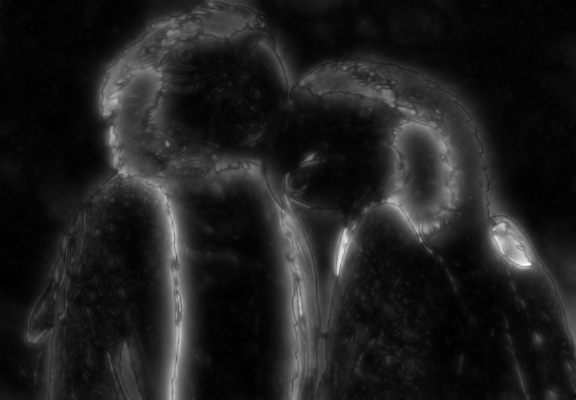
\includegraphics[width=0.3\linewidth]{img/arara_col_map.png}
            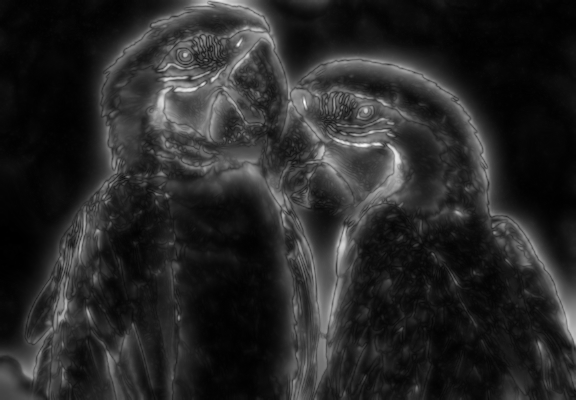
\includegraphics[width=0.3\linewidth]{img/arara_cst_map.png}
            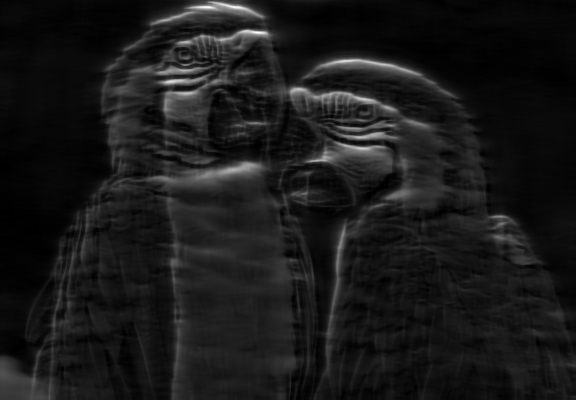
\includegraphics[width=0.3\linewidth]{img/arara_ort_map.png}
		\end{tabular}
\end{center}
\caption{Mapas de saliência da figura original~\ref{fig:extrfeat}.
    Esquerda: mapa de cor. Centro: mapa de luminância. Direita: mapa de
orientação.}
\label{fig:maps}
\end{figure}

\subsubsection{Combinação final}
É dado um peso para cada mapa de saliência (cor, luminância, orientação)
e então eles são somados e normalizados. Nos testes feitos, obteve-se
melhores resultados dando peso maior para a cor e menor para a orientação.
Nos exemplos aqui, os pesos são 2, 1, 0.1 para cor, luminância e orientação,
respectivamente.
\begin{figure}[H]
\begin{center}
        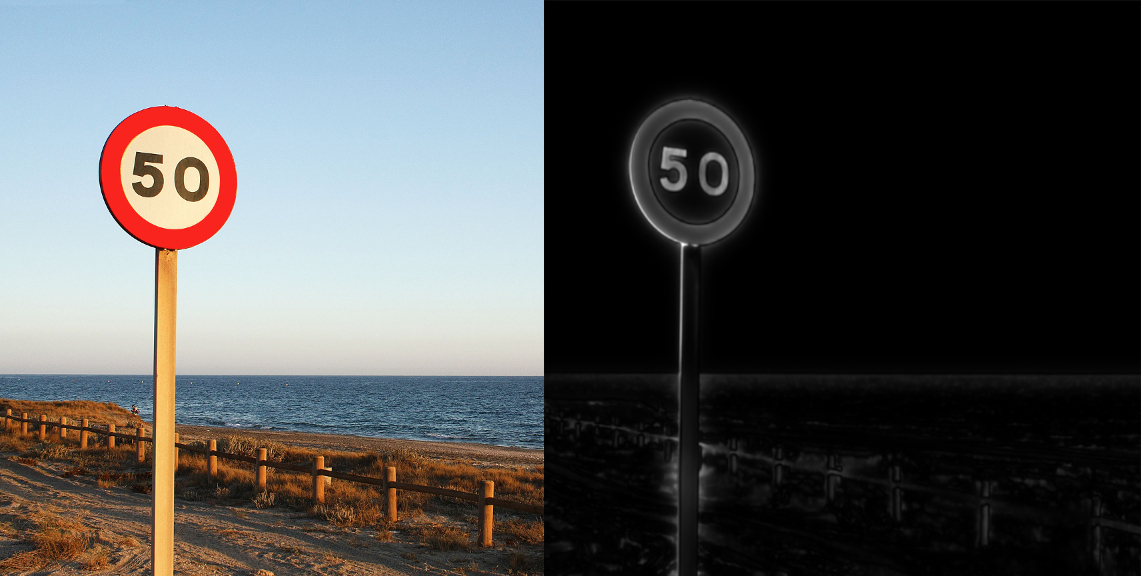
\includegraphics[width=0.6\linewidth]{img/att.png}
\end{center}
\caption{Mapa de saliência final para uma figura. À esquerda, a imagem
    original. À direita, o mapa de saliência final.}
\label{fig:att}
\end{figure}

\subsubsection{Implementação}
Todas as etapas do modelo descritas aqui foram implementadas.
A linguagem utilizada foi \tit{Python}, usando-se \tit{OpenCV} e \tit{numpy}.
O código está disponível de modo público~\cite{att}.

\subsubsection{Considerações}
O modelo implementado foi testado em diversas imagens e dá resultados
satisfatórios na maioria dos casos: em regiões intuitivamente mais salientes,
o mapa mostra a região como mais clara (como na figura~\ref{fig:att}).
Há muitos hiperparâmetros para o modelo, como: níveis de pirâmide,
valores dos filtros de Gabor, método de normalização, pesos para os mapas.
Isso exige buscas exaustivas no espaço de alta dimensionalidade dos
hiperparâmetros para achar bons valores, o que é muito custoso.
Assim, embora o modelo atual dê bons resultados, um ponto negativo
é a alta quantidade de hiperparâmetros.

\subsection{Avaliação de desempenho}
Foi feita uma pesquisa das métricas e \tit{datasets} mais usados para
avaliação dos modelos computacionais, pois isso
é muito importante para o avanço do trabalho.

\subsubsection{\tit{Datasets}}
Os \tit{datasets} são compostos de imagens juntamente ao conjunto-verdade,
algo que indica como os mapas de saliência para cada imagem deveriam ser.

Dois dos tipos principais de mapas-verdade:
\begin{enumerate}
	\item Pontos de fixação de olhar: Algum dispositivo de
	\tit{eye-tracking} é usado em pessoas para determinar as regiões na imagem
	onde as mesmas olham em um intervalo de tempo. Apenas os pixels com
	fixação são brancos.

	\item Máscaras contínuas: As regiões salientes têm valores
	contínuos em um intervalo de intensidade de \tit{pixels}, com valores
	maiores representando uma saliência maior.
	São geralmente obtidas através dos pontos de fixação, aplicando-se
	uma gaussiana adequada em cada ponto.
\end{enumerate}

Alguns \tit{datasets} utilizados geralmente:
\begin{itemize}
	\item \ttt{CAT2000~\cite{cat2000}:} 4000 imagens de 20 categorias com
		dados de fixação de olhar de 24 pessoas por imagem de duração de
		5 segundos.

	\item \ttt{JUDD~\cite{juddBM}:} 1003 imagens de diversos tipos com
		dados de fixação de olhar de 15 pessoas por imagem. Acompanha também
		mapas contínuos. É amplamente usado.

	\item \ttt{MIT300~\cite{mit-300}:} 300 imagens de diversos tipos
		com dados de fixação. Entretanto, os mesmos não estão disponíveis
		e devem ser testados pelos donos do \tit{dataset}.
\end{itemize}

\subsubsection{Métricas}
Muitas das métricas aqui mostradas são discutidas em~\cite{judd2},
onde a aplicabilidade, significado, vantagens e desvantagens
de cada uma são discutidas mais a fundo. Aqui daremos apenas uma breve
descrição das mesmas.

\begin{itemize}
	\item \ttt{AUC-Judd}\newline
	Abreviação de \tit{Area Under ROC Curve}. É feita uma varredura em diversos
	valores de \tit{threshold} para o mapa de saliência e, para cada valor,
	calcula-se o \tit{true positive rate} e o \tit{false positive rate} com
	base na máscara feita para o mapa de saliência e os pixels brancos
	respectivos aos pontos de fixação de humanos.
	A área embaixo da \tit{ROC} formada então é calculada.
	Usado em~\cite{mit-300, juddBM}.

	\item \ttt{NSS}\newline
	\ttt{AUC} pode avaliar com altas pontuações mapas com falsos positivos
	mas com valores baixos nestes falsos positivos~\cite{judd2}.
	O \ttt{NSS} penaliza isso e dá altas pontuações a mapas com valores
	baixos em negativos e altos em positivos:
	$$NSS(P, Q) = \frac{1}{N}\sum\limits_{i=1}^N{\bar{P_{i}}Q_{i}}$$
	Onde $N$ é o número de pontos de fixação,
	$Q$ é o mapa binário de pontos de fixação e $\bar{P}$ é o mapa de
	saliência normalizado pelo desvio padrão.
	Usado em~\cite{mit-300}.

	\item \ttt{Similarity}\newline
	Métrica para mapas contínuos. Definido como:
	$$SIM(P, Q) = \frac{1}{N}\sum\limits_{i=1}^N{min(P_i, Q_i)}$$
	Com $P$ e $Q$ indo de $0$ a $1$. Um valor de $1$ define mapas idênticos
	e $0$ mapas totalmente diferentes.
	Ambos os mapas são normalizados pela soma de cada um.
	Usado em~\cite{mit-300}.

	\item \ttt{Correlation Coefficient}\newline
	Métrica para mapas contínuos.
	\ttt{Similarity} penaliza \tit{false negatives} mais que
	\tit{false positives}~\cite{judd2}. A métrica \ttt{CC} trata os dois
	simetricamente. Dada por:
	$$CC(P, Q) = \frac{cov(P,Q)}{\sigma(P)\sigma(Q)}$$
	Onde $P$ é normalizado no intervalo $[0, 1]$.
	Usado em~\cite{mit-300}.
\end{itemize}

Para \tit{ground-truth} por pontos binários de fixação,
\ttt{AUC} é razoável para casos em que se quer um
bom \tit{recall} e que falsos negativos mas com valores relativamente baixos
não importam muito. Isso é verdade em casos em que o foco atencional será
direcionado apenas à região de maior valor.
\ttt{NSS} também pode ser válido pois ele penaliza falsos positivos mesmo
que baixos, focando mais em \tit{precision}.
Para \tit{ground-truth} contínuos derivados de pontos de fixação,
\ttt{SIM} é bom quando importa-se com \tit{recall}, pois a métrica penaliza
falsos negativos mais que falsos positivos.
\ttt{CC} também é boa por ser neutra e penalizar falsos positivos/negativos
igualmente.

\subsubsection{Comparação com outros modelos}
Foi construído um ambiente de \tit{benchmark} para o modelo \ttt{att},
que permite fazer testes automatizados com diversos \tit{datasets} e métricas.
O primeiro uso deste ambiente foi para fazer uma busca inicial de
hiperparâmetros para o modelo: muitos valores destes diminuíam muito o
desempenho do modelo, alguns aumentando o valor em uma métrica mas
diminuindo consideravelmente em outra. Assim, foi feita uma escolha de
hiperparâmetros que não prejudicasse muito nenhuma métrica.

O conjunto de imagens escolhido foi \ttt{Judd}~\cite{juddBM}.
Com uma amostragem aleatória de 128 imagens, calculamos diversas métricas
e comparamos com modelos presentes na tabela do
\tit{MIT Saliency Benchmark}~\cite{mitsal}, um \tit{benchmark}
amplamente utilizado.
Na comparação aqui mostrada, comparamos nosso modelo com três tipos de
modelos: um que fica consistentemente entre os primeiros para diversas
métricas (\tit{DeepFix}~\cite{DeepFix}), um que fica consistentemente na metade
(\tit{Rosin Saliency 2}~\cite{rosinsal2}),
e um que fica consistentemente entre os últimos (\tit{IttiKoch}~\cite{itti}).
Usamos duas métricas para pontos de saliência (\ttt{AUC-Judd, NSS}) e duas para
mapas contínuos (\ttt{SIM, CC}).
\begin{figure}[H]
%\begin{center}
    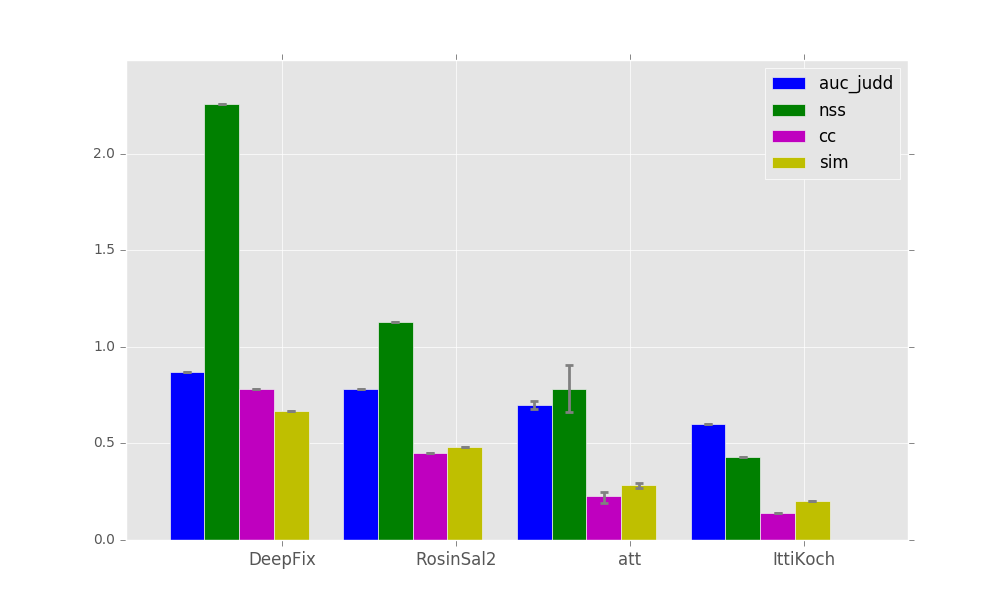
\includegraphics[width=1.1\linewidth]{img/comp.png}
%\end{center}
\caption{Comparação de desempenho do modelo att com diversos modelos
do \tit{MIT Saliency Benchmark}}
\label{fig:comp}
\end{figure}

Nota-se que nosso modelo é superior em todas as métricas ao \tit{IttiKoch},
tem resultados comparáveis (mas sempre piores) ao \tit{Rosin Saliency 2},
e tem resultados muito inferiores aos do \tit{DeepFix}.
Modelos modernos do topo como o \tit{DeepFix} usam técnicas muito diferentes
das usadas pelo nosso modelo, muitas vezes usando \tit{Deep Learning}.
Isso motiva a busca de uma nova abordagem para o nosso modelo.

\section{Próximos passos}
\subsection{Nova versão do modelo att}
Alguns dos modelos computacionais de saliência visual que ficam consistentemente
no topo da lista do \tit{MIT Saliency Benchmark} são:
\tit{DeepFix}~\cite{DeepFix},
\tit{Salicon}~\cite{Salicon}, \tit{Deep Gaze 2}~\cite{DeepGaze2},
\tit{SalNet}~\cite{SalNet}.
O que todos estes têm em comum é o uso de técnicas de \tit{Deep Learning},
com o uso de redes neurais convolucionais.
Ao que tudo indica, modelos usando tais técnicas têm resultados
sempre superiores aos modelos como o VOCUS e a maior parte da comunidade
na área adotou essa abordagem.

Um próximo passo natural para o projeto é aplicar técnicas semelhantes às dos
modelos dominantes.
Uma pesquisa nos modelos do topo foi feita para analisar melhor suas técnicas
e avaliar a possibilidade da implementação de suas ideias.
Com base na boa descrição do modelo e os excelentes resultados, escolheu-se
basear no \tit{DeepFix} para a nova versão do modelo \ttt{att}.
Planeja-se implementar o modelo como um todo -- ou sua maior parte --.

\subsubsection{Extensão para vídeo}
Não há sinal na literatura de algum modelo que foi projetado para funcionar
também em vídeos. A extensão de modelos para vídeos não é imediata, pois
deve-se contar com efeitos como a transição de foco de atenção ao longo do
tempo, um efeito que não existe em imagens.
Assim, faz parte dos próximos passos desenvolver um modo de estender o modelo
novo do \ttt{att} -- baseado no \tit{DeepFix} -- para análise
atencional em vídeos.
Tal contribuição seria inédita até o momento para a área.

\subsection{Construção de \tit{Framework}}
A etapa final é a construção de um \tit{Framework}.
O mesmo será implementado em um robô móvel, onde serão definidas tarefas
de navegação e será feita uma avaliação do desempenho do robô.

\printbibliography

%\end{multicols}
\end{document}
